

\documentclass{report}\usepackage{graphicx, color}
%% maxwidth is the original width if it is less than linewidth
%% otherwise use linewidth (to make sure the graphics do not exceed the margin)
\makeatletter
\def\maxwidth{ %
  \ifdim\Gin@nat@width>\linewidth
    \linewidth
  \else
    \Gin@nat@width
  \fi
}
\makeatother

\IfFileExists{upquote.sty}{\usepackage{upquote}}{}
\definecolor{fgcolor}{rgb}{0.2, 0.2, 0.2}
\newcommand{\hlnumber}[1]{\textcolor[rgb]{0,0,0}{#1}}%
\newcommand{\hlfunctioncall}[1]{\textcolor[rgb]{0.501960784313725,0,0.329411764705882}{\textbf{#1}}}%
\newcommand{\hlstring}[1]{\textcolor[rgb]{0.6,0.6,1}{#1}}%
\newcommand{\hlkeyword}[1]{\textcolor[rgb]{0,0,0}{\textbf{#1}}}%
\newcommand{\hlargument}[1]{\textcolor[rgb]{0.690196078431373,0.250980392156863,0.0196078431372549}{#1}}%
\newcommand{\hlcomment}[1]{\textcolor[rgb]{0.180392156862745,0.6,0.341176470588235}{#1}}%
\newcommand{\hlroxygencomment}[1]{\textcolor[rgb]{0.43921568627451,0.47843137254902,0.701960784313725}{#1}}%
\newcommand{\hlformalargs}[1]{\textcolor[rgb]{0.690196078431373,0.250980392156863,0.0196078431372549}{#1}}%
\newcommand{\hleqformalargs}[1]{\textcolor[rgb]{0.690196078431373,0.250980392156863,0.0196078431372549}{#1}}%
\newcommand{\hlassignement}[1]{\textcolor[rgb]{0,0,0}{\textbf{#1}}}%
\newcommand{\hlpackage}[1]{\textcolor[rgb]{0.588235294117647,0.709803921568627,0.145098039215686}{#1}}%
\newcommand{\hlslot}[1]{\textit{#1}}%
\newcommand{\hlsymbol}[1]{\textcolor[rgb]{0,0,0}{#1}}%
\newcommand{\hlprompt}[1]{\textcolor[rgb]{0.2,0.2,0.2}{#1}}%

\usepackage{framed}
\makeatletter
\newenvironment{kframe}{%
 \def\at@end@of@kframe{}%
 \ifinner\ifhmode%
  \def\at@end@of@kframe{\end{minipage}}%
  \begin{minipage}{\columnwidth}%
 \fi\fi%
 \def\FrameCommand##1{\hskip\@totalleftmargin \hskip-\fboxsep
 \colorbox{shadecolor}{##1}\hskip-\fboxsep
     % There is no \\@totalrightmargin, so:
     \hskip-\linewidth \hskip-\@totalleftmargin \hskip\columnwidth}%
 \MakeFramed {\advance\hsize-\width
   \@totalleftmargin\z@ \linewidth\hsize
   \@setminipage}}%
 {\par\unskip\endMakeFramed%
 \at@end@of@kframe}
\makeatother

\definecolor{shadecolor}{rgb}{.97, .97, .97}
\definecolor{messagecolor}{rgb}{0, 0, 0}
\definecolor{warningcolor}{rgb}{1, 0, 1}
\definecolor{errorcolor}{rgb}{1, 0, 0}
\newenvironment{knitrout}{}{} % an empty environment to be redefined in TeX

\usepackage{alltt}
\usepackage{mparhack}
\usepackage{xstring}

\usepackage{etoolbox}
\usepackage{multicol}
\usepackage{xcolor}


\usepackage[landscape,margin=.25in,bottom=.35in,includehead,includefoot]{geometry}
\usepackage{probstat}
\usepackage{hyperref}
\usepackage{longtable}

\usepackage{tikz}
\usetikzlibrary{shadows}
\usetikzlibrary{decorations}
\usetikzlibrary{shapes.multipart}
\usetikzlibrary{shapes.symbols}
\usetikzlibrary{shapes.misc}
\usetikzlibrary{shapes.geometric}

\newcommand{\mymarginpar}[1]{%
\vadjust{\smash{\llap{\parbox[t]{\marginparwidth}{#1}\kern\marginparsep}}}}


\usepackage[utf8]{inputenc}

\usepackage[Bjornstrup]{fncychap}
\usepackage{fancyvrb}
\usepackage{fancyhdr}
\pagestyle{fancy}
\fancyhf{}

%% Now begin customising things. See the fancyhdr docs for more info.

\renewcommand{\chaptermark}[1]{\thispagestyle{fancy}\markboth{{#1}}{}}
\renewcommand{\sectionmark}[1]{\markright{{#1}}{}}
%\renewcommand{\headrulewidth}{0pt}

\chead{}
\lhead[\sf \thepage]{\sf \leftmark}
\rhead[\sf \leftmark]{\sf \thepage}
%\lfoot[\sf USCOTS 2011]{\sf Teaching Statistics With R}
%\rfoot[\sf Teaching Statistics With R]{\sf USCOTS 2011}
%\cfoot{\sf \copyright 2011, R Pruim, N J Horton and D Kaplan}

\newcounter{myenumi}
\newcommand{\saveenumi}{\setcounter{myenumi}{\value{enumi}}}
\newcommand{\reuseenumi}{\setcounter{enumi}{\value{myenumi}}}

\pagestyle{fancy}


%\usepackage{titlesec}
%\titleformat{\chapter}[block]{\huge \sf \bfseries }{\thechapter}{5mm}{}[] 



\def\R{{\sf R}}
\def\Rstudio{{\sf RStudio}}
\def\RStudio{{\sf RStudio}}
\def\term#1{\textbf{#1}}
\def\tab#1{{\sf #1}}

\usepackage{sfsect}
\usepackage{relsize}
%\usepackage{listings}

\def\myRuleColor{\color{black!50!white}}


\definecolor{GrayBoxGray}{rgb}{0.94,0.95,0.95}
\definecolor{GrayBoxGray}{rgb}{0.97,0.98,0.95}
\colorlet{GrayBoxGray}{blue!10!black!10}
\colorlet{GrayBoxGray}{blue!7}

\newlength{\tempfmlength}
\newsavebox{\fmbox}
\newenvironment{fmpage}[1]
     {
	 \medskip
	 \setlength{\tempfmlength}{#1}
	 \begin{lrbox}{\fmbox}
	   \begin{minipage}{#1}
		 \vspace*{.02\tempfmlength}
		 \hfill
	   \begin{minipage}{.95 \tempfmlength}}
		 {\end{minipage}\hfill
		 \vspace*{.015\tempfmlength}
		 \end{minipage}\end{lrbox}\fbox{\usebox{\fmbox}}
	 \medskip
	 }


\newenvironment{boxedText}[1][.98\textwidth]%
{%
\begin{center}
\begin{fmpage}{#1}
}%
{%
\end{fmpage}
\end{center}
}

\newenvironment{boxedTable}[2][tbp]%
{%
\begin{table}[#1]
  \refstepcounter{table}
  \begin{center}
\begin{fmpage}{.98\textwidth}
  \begin{center}
	\sf \large Box~\expandafter\thetable. #2
\end{center}
\medskip
}%
{%
\end{fmpage}
\end{center}
\end{table}		% need to do something about exercises that follow boxedTable
}



% indexing
\newcommand{\printindex}[1]{\relax}
\newcommand{\indexchap}[1]{\relax}
\usepackage{amsmidx}
\newcommand{\exampleidx}[1]{{\it #1}}
\newcommand{\defidx}[1]{{\bf #1}}
\newcommand{\mainidx}[1]{{\bf #1}}
\newcommand{\probidx}[1]{{{\underline{#1}}}}

\makeindex{Rindex}
\makeindex{mainIndex}
\newcommand{\Rindex}[1]{\index{Rindex}{#1@\texttt{#1}}}
\newcommand{\myindex}[1]{\index{mainIndex}{#1}}
\newcommand{\mathindex}[1]{\index{mainIndex}{$#1$}}

\newcommand{\cran}{\href{http://www.R-project.org/}{CRAN}}

\newcommand{\rterm}[1]{\textbf{#1}}


% Looking for a consistent typography for variable names.
% for consistency, we need to match all the verbatim uses elsewhere 
% unless someone wants to recode all that.
\newcommand{\VN}[1]{{\color{green!50!black}\texttt{#1}}}
\newcommand{\vn}[1]{{\color{green!50!black}\texttt{#1}}}
\newcommand{\variable}[1]{{\color{green!50!black}\texttt{#1}}}
\newcommand{\DFN}[1]{{\color{blue!80!black}\texttt{#1}}}
\newcommand{\dfn}[1]{{\color{blue!80!black}\texttt{#1}}}
\newcommand{\dataframe}[1]{{\color{blue!80!black}\texttt{#1}}}
\newcommand{\function}[1]{{\color{purple!75!blue}\texttt{\StrSubstitute{#1}{()}{}()}}}
\newcommand{\option}[1]{{\color{brown!80!black}\texttt{#1}}}
\newcommand{\pkg}[1]{{\color{red!80!black}\texttt{#1}}}
\renewcommand{\code}[1]{{\color{blue!80!black}\texttt{#1}}}
% and for models
\newcommand{\model}[2]{{$\,$\hbox{#1}\ \ensuremath{\sim}\ \hbox{#2}}}

\newenvironment{comment}{%
\begin{quote}
\em
}{%
\end{quote}
}


\title{Minimal R for Intro Stats}

\author{
Randall Pruim
}

\date{June, 2012}


\begin{document}
\parindent=0pt

\chead{\sf \bfseries \Large Enough R for Intro to Statistical Modeling}
\rhead{September 2012}
\lhead{R. Pruim \& D. Kaplan}













\let\oldchapter=\chapter
\def\chapter{\setcounter{page}{1}\oldchapter}


%\begin{center}
%\section*{Enough R for Intro Stats}
%\end{center}

\def\opt#1{#1}
\def\squeeze{\vspace*{-4ex}}
A couple dozen functions suffice to carry out your work in Introduction to Statistical Modeling.  This sheet provides the names of functions, a review of formula syntax, and some examples of use.

\begin{multicols}{4}
\raggedright

\subsection*{Help}
\begin{knitrout}
\definecolor{shadecolor}{rgb}{0.969, 0.969, 0.969}\color{fgcolor}\begin{kframe}
\begin{alltt}
\hlfunctioncall{help}()
\hlfunctioncall{apropos}()  
?
??
\hlfunctioncall{example}()
\end{alltt}
\end{kframe}
\end{knitrout}


\subsection*{Arithmetic}
Basic arithmetic is very similar to a calculator.
\begin{knitrout}
\definecolor{shadecolor}{rgb}{0.969, 0.969, 0.969}\color{fgcolor}\begin{kframe}
\begin{alltt}
\hlcomment{# basic ops: + - * / ^ ( )}
\hlfunctioncall{log}()
\hlfunctioncall{exp}()
\hlfunctioncall{sqrt}()
\hlfunctioncall{log10}()
\hlfunctioncall{abs}()
\end{alltt}
\end{kframe}
\end{knitrout}


\subsection*{Randomization/Iteration}
%
\begin{knitrout}
\definecolor{shadecolor}{rgb}{0.969, 0.969, 0.969}\color{fgcolor}\begin{kframe}
\begin{alltt}
\hlfunctioncall{do}()        \hlcomment{# mosaic}
\hlfunctioncall{sample}()    \hlcomment{# mosaic augmented}
\hlfunctioncall{resample}()  \hlcomment{# with replacement}
\hlfunctioncall{shuffle}()   \hlcomment{# mosaic}
\end{alltt}
\end{kframe}
\end{knitrout}


\subsection*{Graphics}

%
\begin{knitrout}
\definecolor{shadecolor}{rgb}{0.969, 0.969, 0.969}\color{fgcolor}\begin{kframe}
\begin{alltt}
\hlfunctioncall{bwplot}()
\hlfunctioncall{xyplot}()
\hlfunctioncall{densityplot}()
\hlfunctioncall{histogram}()
\hlfunctioncall{plotFun}() \hlcomment{# mosaic}
\end{alltt}
\end{kframe}
\end{knitrout}


\vfill
\columnbreak

\subsection*{Numerical Summaries}
These functions have 
a formula interface to match plotting.
%
\begin{knitrout}
\definecolor{shadecolor}{rgb}{0.969, 0.969, 0.969}\color{fgcolor}\begin{kframe}
\begin{alltt}
\hlfunctioncall{mean}()   \hlcomment{# mosaic augmented}
\hlfunctioncall{median}() \hlcomment{# mosaic augmented}
\hlfunctioncall{sd}()     \hlcomment{# mosaic augmented}
\hlfunctioncall{var}()    \hlcomment{# mosaic augmented}
\hlfunctioncall{tally}()  \hlcomment{# mosaic}
\hlfunctioncall{qdata}()  \hlcomment{# mosaic}
\hlfunctioncall{pdata}()  \hlcomment{# mosaic}
\hlfunctioncall{IQR}()
\end{alltt}
\end{kframe}
\end{knitrout}


\subsection*{Model Building and Inference}
%
\begin{knitrout}
\definecolor{shadecolor}{rgb}{0.969, 0.969, 0.969}\color{fgcolor}\begin{kframe}
\begin{alltt}
\hlfunctioncall{mm}()      \hlcomment{# mosaic}
\hlfunctioncall{lm}()      \hlcomment{# linear models}
\hlfunctioncall{glm}()     \hlcomment{# for logistic models}
\hlfunctioncall{resid}()
\hlfunctioncall{fitted}()
\hlfunctioncall{confint}()
\hlfunctioncall{anova}()
\hlfunctioncall{summary}()
\hlfunctioncall{makeFun}() \hlcomment{# mosaic }
\hlfunctioncall{listFun}() \hlcomment{# devel}
\end{alltt}
\end{kframe}
\end{knitrout}


\subsection*{Interactive}
For classroom use.
\begin{knitrout}
\definecolor{shadecolor}{rgb}{0.969, 0.969, 0.969}\color{fgcolor}\begin{kframe}
\begin{alltt}
\hlfunctioncall{mLM}()  \hlfunctioncall{mLineFit}()  \hlfunctioncall{mLinAlgebra}()
\hlfunctioncall{mCI}()  \hlfunctioncall{mHypTest}() \hlfunctioncall{mPower}()
\end{alltt}
\end{kframe}
\end{knitrout}



\vfill

\columnbreak

\subsection*{Formulas for Models}
\begin{knitrout}
\definecolor{shadecolor}{rgb}{0.969, 0.969, 0.969}\color{fgcolor}\begin{kframe}
\begin{alltt}
response ~ a+b \hlcomment{# main effects}
response ~ a*b \hlcomment{# interaction, too}
\end{alltt}
\end{kframe}
\end{knitrout}

Do not use \verb+|+ or \verb+groups=+.

\medskip

{\bf Common forms:}

All cases the same:

\verb=response ~ 1=

\medskip

Main effects & intercept 
\verb=response ~ X + Y=

\medskip

Exclude intercept  (Rarely used.  Be careful!)

\verb=response ~ -1 + X + Y=

\medskip

Main effects and interaction:
\verb=response ~ X * Y=

\medskip

Pure interaction (Rarely used.)
\verb=response ~ X:Y=

\medskip

Polynomial terms:
\verb=response ~ poly(X,2)=

\medskip

Random model vectors (pedagogical)
\verb=response ~ rand(2)= 

\subsection*{Data and Variables}
\begin{knitrout}
\definecolor{shadecolor}{rgb}{0.969, 0.969, 0.969}\color{fgcolor}\begin{kframe}
\begin{alltt}
\hlfunctioncall{fetchData}() \hlcomment{# mosaic}
\hlfunctioncall{names}()
\hlfunctioncall{head}()
\hlfunctioncall{levels}()
\hlfunctioncall{subset}()
\hlfunctioncall{with}()      \hlcomment{# operate on data}
\hlfunctioncall{transform}() \hlcomment{# new var in data }
\hlfunctioncall{factor}()    \hlcomment{# categorical vars}
\hlfunctioncall{merge}()
\hlfunctioncall{rank}()
\end{alltt}
\end{kframe}
\end{knitrout}




\vfill

\columnbreak


\subsection*{Formulas for Graphs \& Numerics}
Plotting (e.g. \texttt{xyplot}, \texttt{densityplot}, \texttt{bwplot}) and simple numerics (e.g. \texttt{tally}, \texttt{mm}) use formulas in the following ways:

\begin{knitrout}
\definecolor{shadecolor}{rgb}{0.969, 0.969, 0.969}\color{fgcolor}\begin{kframe}
\begin{alltt}
\hlfunctioncall{fname}( y ~ x | z, data=..., 
                  groups=... )
\end{alltt}
\end{kframe}
\end{knitrout}

\noindent \texttt{y}: is y-axis variable.  Leave blank for densityplots 

\noindent \texttt{x}: is x-axis variable
  
\noindent \texttt{z}: conditioning variable (separate panes in graphs)
	
\noindent  \texttt{groups}: conditioning variable (overlaid in graphs)

For other things y ~ x | z
 can usually be read y
 or depends on x
 separately for each z
.

\subsection*{Common Example Datasets}
Can be used directly with \texttt{data=}:
\begin{knitrout}
\definecolor{shadecolor}{rgb}{0.969, 0.969, 0.969}\color{fgcolor}\begin{kframe}
\begin{alltt}
Galton       \hlcomment{# heights}
CPS85        \hlcomment{# wages}
KidsFeet
Marriage
SAT
\end{alltt}
\end{kframe}
\end{knitrout}


Read in with \texttt{fetchData()}:
\begin{knitrout}
\definecolor{shadecolor}{rgb}{0.969, 0.969, 0.969}\color{fgcolor}\begin{kframe}
\begin{alltt}
utils = \hlfunctioncall{fetchData}(\hlstring{"utilities.csv"})
alder = \hlfunctioncall{fetchData}(\hlstring{"alder.csv"})
grades = \hlfunctioncall{fetchData}(\hlstring{"grades.csv"})
courses = \hlfunctioncall{fetchData}(\hlstring{"courses.csv"})
\hlcomment{# Load software in development:}
\hlfunctioncall{fetchData}(\hlstring{"m155development.R"})
\end{alltt}
\end{kframe}
\end{knitrout}



\vfill

\end{multicols}

\newpage

\chead{\sf \bfseries \Large R Sampler for Intro to Statistical Modeling}

\def\opt#1{#1}
\def\squeeze{\vspace*{-4ex}}

\begin{multicols}{4}
\footnotesize




\subsection*{Quick Look at a Data Frame}

\vspace*{-.1in}
\begin{knitrout}
\definecolor{shadecolor}{rgb}{0.969, 0.969, 0.969}\color{fgcolor}\begin{kframe}
\begin{alltt}
cps = \hlfunctioncall{fetchData}(\hlstring{"CPS85"})
\hlfunctioncall{names}(cps)   \hlfunctioncall{nrow}(cps)    \hlfunctioncall{summary}(cps)  
\hlfunctioncall{head}(cps)    \hlfunctioncall{sample}(cps,size=5)
\end{alltt}
\end{kframe}
\end{knitrout}


\vspace*{-.2in}

\subsection*{Tallying}
A simple count of the number in each level

\vspace*{-.1in}

\begin{knitrout}
\definecolor{shadecolor}{rgb}{0.969, 0.969, 0.969}\color{fgcolor}\begin{kframe}
\begin{alltt}
\hlfunctioncall{tally}(~sex, data = CPS85)
\end{alltt}
\end{kframe}
\end{knitrout}

A two-way table of counts

\vspace*{-.1in}

\begin{knitrout}
\definecolor{shadecolor}{rgb}{0.969, 0.969, 0.969}\color{fgcolor}\begin{kframe}
\begin{alltt}
\hlfunctioncall{tally}(~sex + married, data = CPS85)
\end{alltt}
\end{kframe}
\end{knitrout}


\vspace*{-.1in}
Conditional proportions: A $|$ B means ``A conditioned on B".

\vspace*{-.1in}
\begin{knitrout}
\definecolor{shadecolor}{rgb}{0.969, 0.969, 0.969}\color{fgcolor}\begin{kframe}
\begin{alltt}
\hlfunctioncall{tally}(~sex | married, data = CPS85)
\end{alltt}
\end{kframe}
\end{knitrout}


\vspace*{-.1in}

Different from \verb+~married|sex+.

\subsection*{New Dataframe Variable}

\vspace*{-.2in}

\begin{knitrout}
\definecolor{shadecolor}{rgb}{0.969, 0.969, 0.969}\color{fgcolor}\begin{kframe}
\begin{alltt}
g = \hlfunctioncall{fetchData}(\hlstring{"Galton"})
\end{alltt}
\end{kframe}
\end{knitrout}

Add a variable named \texttt{mid}

\vspace*{-.1in}

\begin{knitrout}
\definecolor{shadecolor}{rgb}{0.969, 0.969, 0.969}\color{fgcolor}\begin{kframe}
\begin{alltt}
g = \hlfunctioncall{transform}(g,
     mid=(father+1.08*mother)/2)
\hlfunctioncall{names}(g)  \hlcomment{#confirm that it's there}
\end{alltt}
\begin{verbatim}
[1] "family" "father" "mother" "sex"   
[5] "height" "nkids"  "mid"   
\end{verbatim}
\end{kframe}
\end{knitrout}


\vspace*{-.2in}

\subsection*{Subsets}
Sometimes you want only part of a data set.

\vspace*{-.1in}

\begin{knitrout}
\definecolor{shadecolor}{rgb}{0.969, 0.969, 0.969}\color{fgcolor}\begin{kframe}
\begin{alltt}
boys = \hlfunctioncall{subset}(KidsFeet, sex==\hlstring{"B"})
elig = \hlfunctioncall{subset}(CPS85, 
        wage>10 & married==\hlstring{"Single"})
pros = \hlfunctioncall{subset}(CPS85, 
  sector %in% \hlfunctioncall{c}(\hlstring{"prof"},\hlstring{"manag"}))
\end{alltt}
\end{kframe}
\end{knitrout}

{\bf ... Random subset}

\vspace*{-.1in}
\begin{knitrout}
\definecolor{shadecolor}{rgb}{0.969, 0.969, 0.969}\color{fgcolor}\begin{kframe}
\begin{alltt}
\hlfunctioncall{subset}(CPS85, size = 4)
\end{alltt}
\end{kframe}
\end{knitrout}


\vspace*{-.2in}

\subsection*{Data from Google Spreadsheets}
In Google, choose {\sc File/Publish to the Web}.
Get link to the published data as CSV, sheet 1.  
Copy the link

\vspace*{-.1in}
\begin{knitrout}
\definecolor{shadecolor}{rgb}{0.969, 0.969, 0.969}\color{fgcolor}\begin{kframe}
\begin{alltt}
mydat=\hlfunctioncall{fetchGoogle}(\hlstring{"https://docs.google..."})
\end{alltt}
\end{kframe}
\end{knitrout}


\vfill
\columnbreak

\subsection*{Distributions}
Simple distribution
\begin{knitrout}
\definecolor{shadecolor}{rgb}{0.969, 0.969, 0.969}\color{fgcolor}\begin{kframe}
\begin{alltt}
\hlfunctioncall{densityplot}(~age, data = CPS85)
\end{alltt}
\end{kframe}
\end{knitrout}

Overlaying two (or more) groups
\begin{knitrout}
\definecolor{shadecolor}{rgb}{0.969, 0.969, 0.969}\color{fgcolor}\begin{kframe}
\begin{alltt}
\hlfunctioncall{densityplot}( ~ age, groups=sex, 
             data=CPS85, auto.key=TRUE)
\end{alltt}
\end{kframe}

{\centering 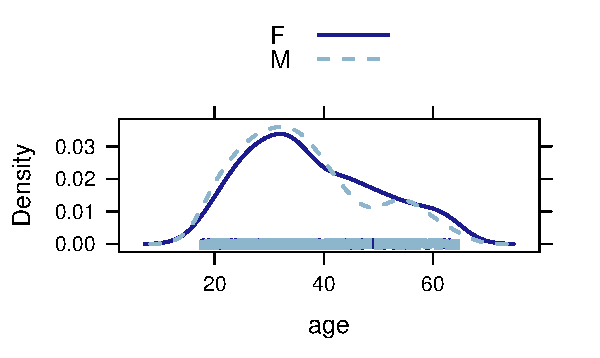
\includegraphics[width=.25\textwidth]{figuresdensityplot2} 

}


\end{knitrout}

\vspace*{-.2in}
Side-by-side plots:
\begin{knitrout}
\definecolor{shadecolor}{rgb}{0.969, 0.969, 0.969}\color{fgcolor}\begin{kframe}
\begin{alltt}
\hlfunctioncall{densityplot}(~age | sex, data = CPS85)
\end{alltt}
\end{kframe}
\end{knitrout}

\vspace*{-.2in}
\begin{knitrout}
\definecolor{shadecolor}{rgb}{0.969, 0.969, 0.969}\color{fgcolor}\begin{kframe}
\begin{alltt}
\hlfunctioncall{bwplot}(age ~ sector, data = CPS85)
\end{alltt}
\end{kframe}
\end{knitrout}


\vspace*{-.2in}

\subsection*{Scatter Plots}

\vspace*{-.1in}
\begin{knitrout}
\definecolor{shadecolor}{rgb}{0.969, 0.969, 0.969}\color{fgcolor}\begin{kframe}
\begin{alltt}
\hlfunctioncall{xyplot}(wage ~ age, data = CPS85)
\end{alltt}
\end{kframe}
\end{knitrout}

\texttt{groups=} and \texttt{|} work as with \texttt{densityplot()}.

\subsection*{Plotting Model Values}

\vspace*{-.1in}

\begin{knitrout}
\definecolor{shadecolor}{rgb}{0.969, 0.969, 0.969}\color{fgcolor}\begin{kframe}
\begin{alltt}
mod = \hlfunctioncall{lm}(wage ~ educ+sex,data=CPS85 )
\hlfunctioncall{xyplot}(\hlfunctioncall{fitted}(mod) ~ educ,data=CPS85 )
\hlfunctioncall{xyplot}(wage+\hlfunctioncall{fitted}(mod) ~ educ,data=CPS85)
\end{alltt}
\end{kframe}
\end{knitrout}


\vspace*{-.2in}

\subsection*{Extract Model Information}

\vspace*{-.1in}

\begin{knitrout}
\definecolor{shadecolor}{rgb}{0.969, 0.969, 0.969}\color{fgcolor}\begin{kframe}
\begin{alltt}
mod = \hlfunctioncall{lm}(wage ~ educ + sex, data = CPS85)
\hlfunctioncall{coef}(mod)
\hlfunctioncall{fitted}(mod)
\hlfunctioncall{resid}(mod)
f = \hlfunctioncall{makeFun}(mod)  \hlcomment{# model function}
\end{alltt}
\end{kframe}
\end{knitrout}

\vfill
\columnbreak

\subsection*{P's and Q's}
Want to find the value that separates the lower 30\% from the higher 70\%:

\vspace*{-.1in}

\begin{knitrout}
\definecolor{shadecolor}{rgb}{0.969, 0.969, 0.969}\color{fgcolor}\begin{kframe}
\begin{alltt}
\hlfunctioncall{qdata}(0.3, wage, data = CPS85)
\end{alltt}
\end{kframe}
\end{knitrout}

Have a value and want to find what fraction of the cases are at or below the value:

\vspace*{-.1in}

\begin{knitrout}
\definecolor{shadecolor}{rgb}{0.969, 0.969, 0.969}\color{fgcolor}\begin{kframe}
\begin{alltt}
\hlfunctioncall{pdata}(10, wage, data = CPS85)
\end{alltt}
\end{kframe}
\end{knitrout}


\vspace*{-.2in}

\subsection*{Randomization}
Sample

\vspace*{-.1in}
\begin{knitrout}
\definecolor{shadecolor}{rgb}{0.969, 0.969, 0.969}\color{fgcolor}\begin{kframe}
\begin{alltt}
mysamp = \hlfunctioncall{sample}(CPS85, size = 100)
\end{alltt}
\end{kframe}
\end{knitrout}


\vspace*{-.1in}

Resample:

\vspace*{-.1in}

\begin{knitrout}
\definecolor{shadecolor}{rgb}{0.969, 0.969, 0.969}\color{fgcolor}\begin{kframe}
\begin{alltt}
\hlfunctioncall{lm}(wage~educ,data=\hlfunctioncall{resample}(CPS85))
\end{alltt}
\end{kframe}
\end{knitrout}


\vspace*{-.1in}

Shuffle (for hypothesis testing)

\vspace*{-.1in}

\begin{knitrout}
\definecolor{shadecolor}{rgb}{0.969, 0.969, 0.969}\color{fgcolor}\begin{kframe}
\begin{alltt}
\hlfunctioncall{lm}(wage~\hlfunctioncall{shuffle}(educ),data=CPS85)
\end{alltt}
\end{kframe}
\end{knitrout}


Probability distributions:

\vspace*{-.1in}

\begin{knitrout}
\definecolor{shadecolor}{rgb}{0.969, 0.969, 0.969}\color{fgcolor}\begin{kframe}
\begin{alltt}
\hlfunctioncall{rnorm}(10,mean=25,sd=2)
\hlfunctioncall{rbinom}(10,prob=.5,size=40)
\hlfunctioncall{rpois}(10,lambda=50) \hlcomment{# events per period}
\hlfunctioncall{rexp}(10,rate=0.01) \hlcomment{# 1/ave time btw events}
\end{alltt}
\end{kframe}
\end{knitrout}

\vspace*{-.1in}

\subsection*{Confidence Intervals}
 {\bf ... via ``normal theory"}

\vspace*{-.1in}

\begin{knitrout}
\definecolor{shadecolor}{rgb}{0.969, 0.969, 0.969}\color{fgcolor}\begin{kframe}
\begin{alltt}
mod = \hlfunctioncall{lm}( wage ~ educ, data=CPS85 )
\hlfunctioncall{confint}(mod)
\end{alltt}
\begin{verbatim}
              2.5 % 97.5 %
(Intercept) -2.7997 1.3077
educ         0.5958 0.9051
\end{verbatim}
\end{kframe}
\end{knitrout}

See also \texttt{summary(mod)}.

\bigskip

 {\bf ... via bootstrapping}

\vspace*{-.1in}

\begin{knitrout}
\definecolor{shadecolor}{rgb}{0.969, 0.969, 0.969}\color{fgcolor}\begin{kframe}
\begin{alltt}
s = \hlfunctioncall{do}(500)*
  \hlfunctioncall{lm}(wage~educ, data=\hlfunctioncall{resample}(CPS85))
\hlfunctioncall{sd}(s) \hlcomment{# standard error}
\end{alltt}
\begin{verbatim}
Intercept      educ     sigma r.squared 
  1.05120   0.08648   0.28221   0.02799 
\end{verbatim}
\end{kframe}
\end{knitrout}

See also \texttt{confint(s)}
\vill
\columnbreak

\subsection*{Quantitative $\rightarrow$ Categorical}
\begin{knitrout}
\definecolor{shadecolor}{rgb}{0.969, 0.969, 0.969}\color{fgcolor}\begin{kframe}
\begin{alltt}
\hlfunctioncall{bwplot}( height ~ \hlfunctioncall{factor}(nkids), 
        data=Galton )
\end{alltt}
\end{kframe}

{\centering \includegraphics[width=.25\textwidth]{figuresunnamed-chunk-31} 

}


\end{knitrout}


\subsection*{Sums of Squares, Dot Products}
\begin{knitrout}
\definecolor{shadecolor}{rgb}{0.969, 0.969, 0.969}\color{fgcolor}\begin{kframe}
\begin{alltt}
\hlfunctioncall{sum}( \hlfunctioncall{fitted}(mod)^2 )
\hlfunctioncall{sum}( \hlfunctioncall{resid}(mod)^2 )
\hlfunctioncall{with}( data=CPS85, \hlfunctioncall{sum}(wage^2))
\hlfunctioncall{sum}(\hlfunctioncall{fitted}(mod)*\hlfunctioncall{resid}(mod)) \hlcomment{# dot prod}
\end{alltt}
\end{kframe}
\end{knitrout}



\subsection*{Something is Wrong}


\begin{knitrout}
\definecolor{shadecolor}{rgb}{0.969, 0.969, 0.969}\color{fgcolor}\begin{kframe}
\begin{alltt}
run = \hlfunctioncall{fetchData}(\hlstring{"repeat-runners.csv"})
\hlfunctioncall{mean}(net, data = run)
\end{alltt}
\begin{verbatim}
[1] NA
\end{verbatim}
\end{kframe}
\end{knitrout}

Some of the data was missing, thus the NA.

{\bf The FIX}:
\begin{knitrout}
\definecolor{shadecolor}{rgb}{0.969, 0.969, 0.969}\color{fgcolor}\begin{kframe}
\begin{alltt}
\hlfunctioncall{options}(na.rm = TRUE)
\hlfunctioncall{mean}(net, data = run)
\end{alltt}
\begin{verbatim}
[1] 88.27
\end{verbatim}
\end{kframe}
\end{knitrout}


\subsection*{Can't Find Something Here?}

Send a note to \verb+kaplan@macalester.edu+




\vfill
\end{multicols}

\end{document}


